El componente electrónico de votación en India, llamado EVM, está compuesto por dos partes: la unidad de votación (izquierda) y la unidad de control (derecha) que están enlazadas por un cable de 5 metros. Las unidades de votación están realizadas para soportar hasta 16 candidatos. En caso de ser más candidatos, se agrega otra unidad de votación y es posible agregar hasta 4 unidades de votación, dando una capacidad máxima de 64 posibles candidatos. En la unidad de votación, se agrega una hoja indicando que botón representa a cada candidato con el símbolo de su partido político. Para votar, el elector tiene que ser identificado por el presidente de mesa que luego le realiza una marca en el dedo con tinta indeleble para evitar que vuelva a votar y presiona un botón en la unidad de control, permitiendo al elector votar en la unidad de votación. Al realizar esto, se prende una luz en la unidad de votación indicando que el votante está listo para sufragar.

\begin{figure}[h]
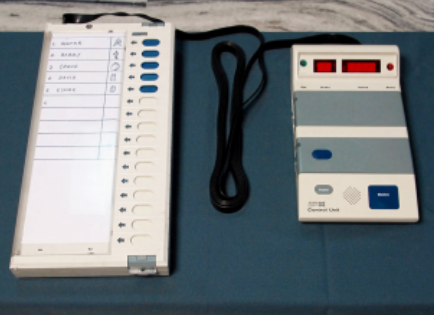
\includegraphics{Imagenes/almacenamiento1}
\caption{Máquina de votación electrónica utilizada en India}
\end{figure}

Las vulnerabilidad encontrada en el paper leído es
\footnote{\url{https://jhalderm.com/pub/papers/evm-ccs10.pdf}}
que se puede reemplazar fácilmente algún componente del equipo sea CPU, placas o agregar hardware. Los diseñadores de las EVM podrían haber hecho los ataques más difíciles agregando un mecanismo criptográfico para identificar a los distintos componentes de hardware originales, como un mecanismo de challenge response basado en un secreto contenido en el firmware original.

Uno de los posibles ataques mencionados en el paper es Dishonest Display. Se desarrolló una placa de visualización que puede reemplazar a la placa real en la unidad de control. Normalmente, cuando los votos son contados, la cantidad de votos recibidos por cada candidato figura en el tablero real. Con el ataque, el tablero agrega un microcontrolador que intercepta los votos totales y realiza la sustitución fraudulenta de resultados emitiéndose en el tablero de visualización. Notar que en este ataque hay que realizar un intercambio de un componente de hardware.

\begin{figure}[h]
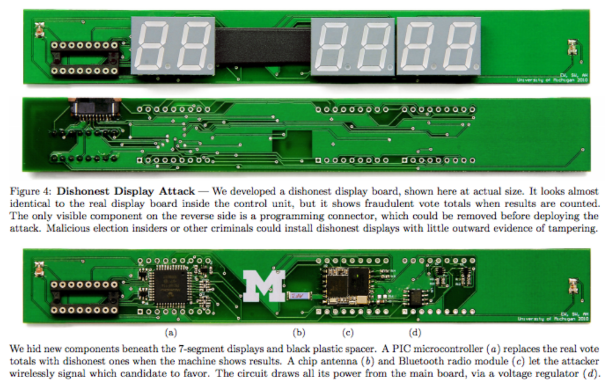
\includegraphics[width=0.8\textwidth]{Imagenes/almacenamiento2}
\caption{Hardware utilizado}
\end{figure}

Un detalle no menor, es que el recuento de votos de la elección en India se realiza semanas después del sufragio. Por ende, el atacante tiene tiempo para poder realizar el cambio o agregar hardware que le permite realizar el ataque mientras están almacenadas.
